\section{第02章 ソフトウェアアーキテクチャ}
\noindent\textbf{この資料の主張}\par
ソフトウェアアーキテクチャは、単なる「大まかな設計図」ではない。アーキテクチャは、ソフトウェア集約システムにおいて根本的であり、後から変えにくく、多くの品質や費用に影響する構造・関係・原則・重要な意思決定の集合である。よいアーキテクチャは、利害関係者の関心事を整理し、設計・実装・テスト・運用・保守に関わる人々が同じ理解を持つための土台になる。

\begin{statementbox}{この資料の読み方}
専門用語は原則として日本語で示し、必要に応じて英語を括弧内に併記する。英語名は、元資料、規格、ツール、文献で同じ概念を確認するための手がかりとして残す。初学者が前提知識なしに読めるように、各節では「何のための概念か」「実務では何を判断するのか」を重視する。
\end{statementbox}

\subsection*{全体概要：この章で学ぶこと}
\addcontentsline{toc}{subsection}{全体概要：この章で学ぶこと}
この章は、ソフトウェアの根本的な形を決め、関係者が共有し、後工程の判断に使うための「アーキテクチャ」を扱う。ここでいうアーキテクチャは、クラス図や構成図そのものではない。図や文書は、アーキテクチャを表すための手段である。アーキテクチャの中心にあるのは、主要な構成要素、それらの関係、設計と進化の原則、品質特性に関するトレードオフ、そして重要な意思決定である。

\noindent\textbf{到達目標}\quad この章を読み終えると、次のことができるようになる。
\begin{itemize}
  \item 「アーキテクチャ」という語が、分野、活動、成果物の三つの意味で使われることを説明できる。
  \item 利害関係者と関心事を分けて考え、アーキテクチャが誰の何に答えるものかを説明できる。
  \item ビューとビューポイントの違いを説明し、複数の図やモデルを使う理由を説明できる。
  \item アーキテクチャ様式、アーキテクチャパターン、参照アーキテクチャを区別できる。
  \item アーキテクチャ設計を、分析、統合、評価の反復活動として説明できる。
  \item アーキテクチャ評価、レビュー、測度の目的を説明できる。
\end{itemize}

\noindent\textbf{学習順序}\quad 初学者は、まず「アーキテクチャとは何か」と「利害関係者と関心事」を押さえる。その後、「どう記述するか」「どう設計するか」「どう評価するか」という流れで読むとよい。

\begin{figure}[htbp]
\centering
\IfFileExists{assets/generated_figures/ch02/fig-ch02-01.png}{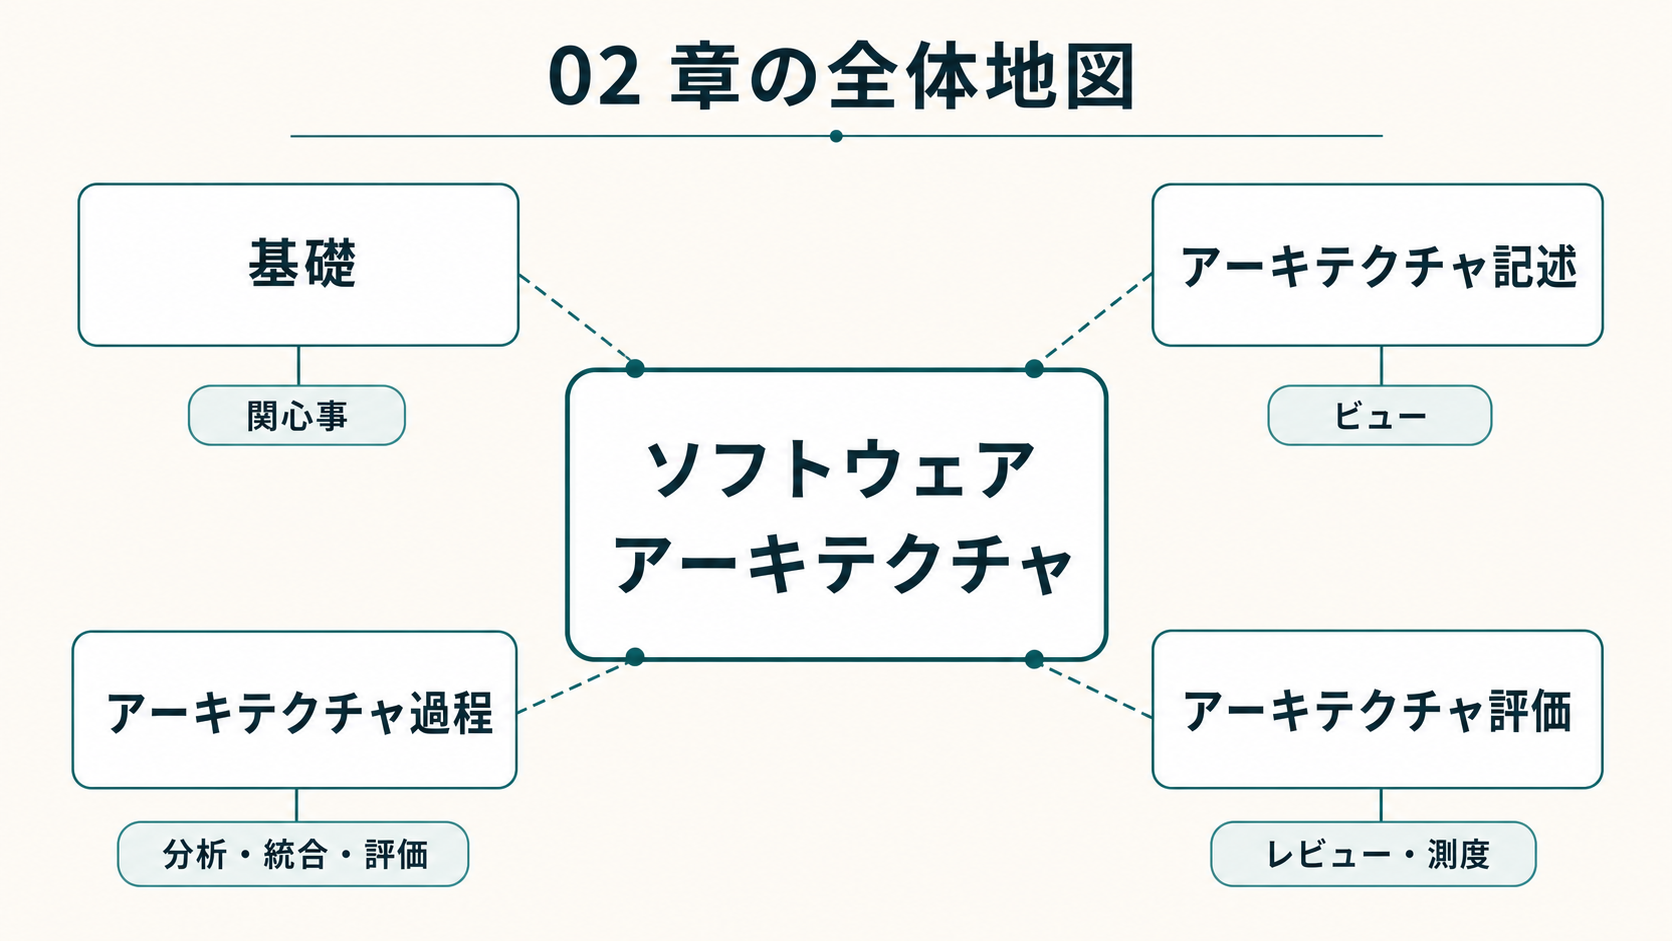
\includegraphics[width=0.96\linewidth]{assets/generated_figures/ch02/fig-ch02-01.png}}{\fbox{\parbox[c][48mm][c]{0.9\linewidth}{\centering 画像生成待ち\\02 章の全体地図}}}
\caption{02 章の全体地図}
\label{fig:ch02-01}
\end{figure}

\subsubsection*{最初に必要な用語}
\addcontentsline{toc}{subsubsection}{最初に必要な用語}
\par\smallskip\noindent\refstepcounter{table}\label{tab:ch02-01}\textbf{表 \thetable: 第02章 ソフトウェアアーキテクチャ 表01}\par\smallskip
\begin{longtable}{P{0.28\linewidth}P{0.64\linewidth}}
\toprule
用語 & 初学者向けの説明 \\
\midrule
ソフトウェア集約システム & ソフトウェアが主要な役割を持つシステムである。ソフトウェアだけでなく、ハードウェア、人、手順、外部サービスも含み得る。 \\
アーキテクチャ & システムの根本的な概念、構成要素、関係、設計と進化の原則である。単なる図ではなく、重要な判断の集合でもある。 \\
利害関係者 & システムに影響を与える、または影響を受ける人や組織である。顧客、利用者、開発者、運用者、保守担当、監査者などが含まれる。 \\
関心事 & 利害関係者が気にする論点である。費用、納期、性能、信頼性、安全性、セキュリティ、使いやすさ、保守しやすさなどである。 \\
品質特性 & システムがどの程度よく振る舞うかを表す性質である。可用性、変更容易性、性能、信頼性、試験容易性などが例である。 \\
アーキテクチャ記述 & アーキテクチャを関係者が使えるように、文書、図、表、モデル、意思決定記録などで表した成果物である。 \\
ビュー & アーキテクチャの一面を表す図やモデルである。論理ビュー、配置ビュー、開発ビューなどがある。 \\
ビューポイント & ビューを作り、読み、使うための規約である。記法、表す要素、関心事、想定読者などを定める。 \\
アーキテクチャ上重要な要求 & アーキテクチャに影響する要求である。英語では Architecturally Significant Requirement、略して ASR と呼ぶ。 \\
アーキテクチャ技術的負債 & 今のアーキテクチャ判断が、将来の変更・運用・保守に追加費用を生む状態である。 \\
\bottomrule
\end{longtable}

\subsection*{導入：なぜソフトウェアアーキテクチャを独立して学ぶのか}
\addcontentsline{toc}{subsection}{導入：なぜソフトウェアアーキテクチャを独立して学ぶのか}
SWEBOK v4.0a では、ソフトウェアアーキテクチャをソフトウェア設計から独立した知識領域として扱う。これは、1990 年代以降にアーキテクチャ研究と実務が大きく発展し、設計の一部としてだけでは説明しきれない知識が増えたためである。

ソフトウェアアーキテクチャは、概念、表現、作業成果物、文脈、過程、方法、分析、評価という複数の視点から理解する必要がある。特に大規模なシステムでは、個々の実装詳細よりも先に、主要な構成要素、構成要素間の関係、外部環境との相互作用、品質特性への対応、変更に対する耐性を考える必要がある。

\begin{statementbox}{重要}
アーキテクチャは「実装の前に一度だけ描く図」ではない。要求、品質、組織、運用、保守、将来の進化に関わる継続的な判断の集合である。
\end{statementbox}
